\section{Overview}

The experiments run for a period of 100 days, from the August 1st 2013 to November 9th, 2013. During this period, we collected 9.5 GB of raw HTTP requests, consisting in approximately 11.0M GET and 1.9M POST. Our honeypots were visited by more than 73,000 different IP addresses, spanning 178 countries and presenting themselves with more than 11,000 distinct User-Agents. This is over one order of magnitude larger than what has been observed in the previous study by John et al. on low interaction web-application honeypots \cite{johnhsh}. Moreover, we also extracted over 110,000 files that were uploaded or modified during attacks against our web sites, 85,000 of them are unique.
There are two different ways to look at the data we collected: one is to identify and study the attacks looking at the web server logs, and the other one is to try to associate a goal to each of them by analyzing the uploaded and modified files. In the first part of this chapter we will look at the first part, while in the second we will give some examples of uploaded files, in order to understand attacker's goals.

\textcolor{blue}{NOTE: maybe remove Overview, as it's closed in itself (we are starting with another section for obtaining nice subsections based on the different phases)}

\section{Exploitation and Post-Exploitation Behaviors}

While analyzing the behavior of attackers lured by our honeypots, we identified four different phases commonly present in an attack session: discovery, reconnaissance, exploitation, and post-exploitation. The \emph{Discovery} phase describes how attackers find their targets, e.g. by querying a search engine (using a dork) or by simply scanning IP addresses. The \emph{Reconnaissance} phase contains information related to the way in which the pages were visited, for instance by using automated crawlers or by manual access, and if this manual access is performed via visual browser or command line tool, and if the attacker is using an anonymization proxy. In the \emph{Exploitation} phase we describe the number and types of actual attacks performed against our web applications. Some of the attacks reach their final goal themselves (for instance by changing a page to redirect to a malicious website), while others are only uploading a second stage. In this case, the uploaded file is often a web shell that is later used by the attacker to manually log in to the compromised system and continue the attack. We refer to this later stage as the \emph{Post-Exploitation} phase.

It must be noticed, however, that not all phases are present in every attack: some of them can be joined in one step (e.g., reconnaissance and exploitation are often performed in one single action), some of them are simply not present (e.g, post-exploitation), some visits do not lead to an actual attack (error in attackers requests, or incomplete file upload), and sometimes it is just impossible to link together different actions performed by the same attacker with different IP addresses.

Neverthless, by extracting the most common patterns from the data collected at each stage, we can identify the ``typical attack profile'' observed during our experiments with the following sequence:

\begin{enumerate}
\item
69.8\% of the attacks start with a scout bot visiting the page. The scout often tries to hide its User Agent (removing directly the header) or disguise themselves as a crawler search (the most used being \emph{GoogleBot});
\item
Few seconds after the scout has identified the page as an interesting target, a second automated system (hereinafter exploitation bot) visits the page and executes the real exploit. This is often a separate script that does not fake the user agent, therefore often appearing with strings such as \emph{libwww/perl}.
\item
If the vulnerability allows the attacker to upload a file, in 46\% of the cases the exploitation bot uploads a web shell. Moreover, the majority of the attacks upload the same file multiple times (in average 9, and sometimes up to 40), probably to be sure that the attack was successful.
\item
After an average of 3 hours and 26 minutes, the attacker logs into the machine using the previously uploaded shell. The average login time for an attacker interactive session is 5 minutes and 37 seconds.
\end{enumerate}

While this represents the most common behavior extracted from our dataset, many other combinations were observed as well - some of which are described in the rest of the section. Finally, it is important to mention that the attack behavior may change depending on the application and on the vulnerability that is exploited. Therefore, we should say that the previous description summarizes the most common behavior of attacks against osCommerce 2.2 (the web application that received by far the largest number of attacks among our honeypots). A particular notice must be performed regarding the SMF application: this application suffered from heavy traffic, provoked by automated bots, and we preferred to exclude this application from our statistics in order to produce more reliable results. A specific discussion over the content of messages posted on the forum will be performed later. In figure ~\ref{fig:overview_phases} we show an overview of the four phases and its characteristics.

\begin{figure}[tbh]
\centerline{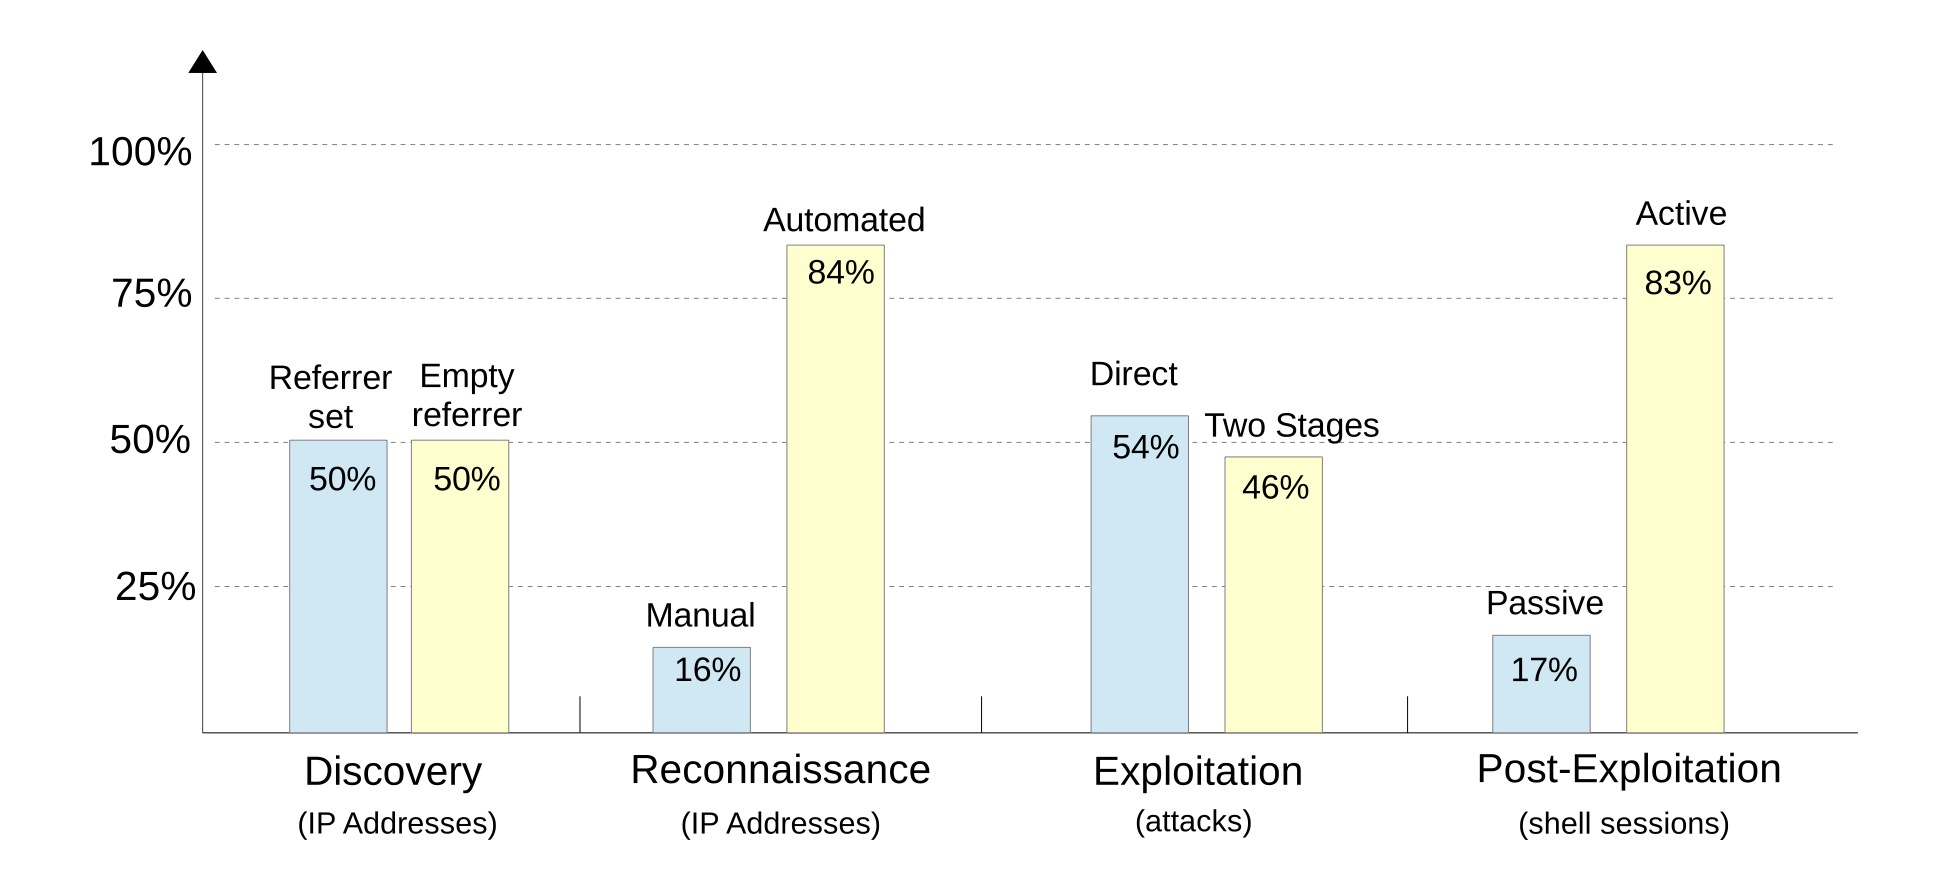
\includegraphics[scale=0.4]{Images/overview_phases.jpg}}
\caption{Overview of the four phases of an attack\label{fig:overview_phases}}
\end{figure}

\subsection{Discovery}
The very first HTTP request hit our HoneyProxy only 10 minutes after the deployment, from ``Googlebot''. The first request not related to a benign crawler came after 1 hour and 50 minutes.
During the first few days, most of the traffic was caused by benign web crawlers. Therefore, we designed a simple solution to filter out benign crawler-generated traffic from the remaining traffic. Since HTTP headers alone are not trustable (e.g., attackers often use User Agents such as ``Googlebot'' in their scripts) we collected public information available on bots and we combined them with information extracted from our logs and validated with WHOIS results in order to identify crawlers from known companies. By combining User Agent strings and the IP address ranges associated to known companies, we were able to identify with certainty 14 different crawlers, originating from 1965 different IPs. Even though this is not a complete list, it was able to successfully filter out most of the traffic generated by benign crawlers.

Some statistics about the origin of the requests is shown in \textcolor{blue}{ADD A GRAPH, TWO LINES WITH DATES, KNOWN CRAWLER AND TOTAL REQUESTS}. The amount of legitimate crawler requests is more or less stable in time, while, as time goes by and the honeypot websites get indexed by search engines and linked on hacking forums or on link farming networks, the number of requests by malicious bots or non-crawlers has an almost linear increase.
While looking at these statistics we also noticed a number of suspicious spikes in the number of accesses. In several cases, one of our web applications was visited, in few hours, by several thousands of unique IP addresses (compared with an average of 192 per day), a clear indication that a botnet was used to scan our sites.

Interestingly, we observed the first suspicious activity only 2 hours and 10 minutes after the deployment of our system, when our forum web application started receiving few automated registrations. However, the first posts on the forum appeared only four days later, on December 27th. Even more surprising was the fact that the first visit from a non-crawler coincided with the first attack: 4 hours 30 minutes after the deployment of the honeypots, a browser with Polish locale visited our osCommerce web application and exploited a file upload vulnerability to upload a malicious PHP script to the honeypot. We also examined the IP source address in order to understand the more active countries, as we can see from ~\ref{fig:requests_countries} Russia, Ukraine and USA are in order the top three countries for number of requests. \textcolor{blue}{HEATMAP OR PIE CHART?}.

\begin{figure}[tbh]
\centerline{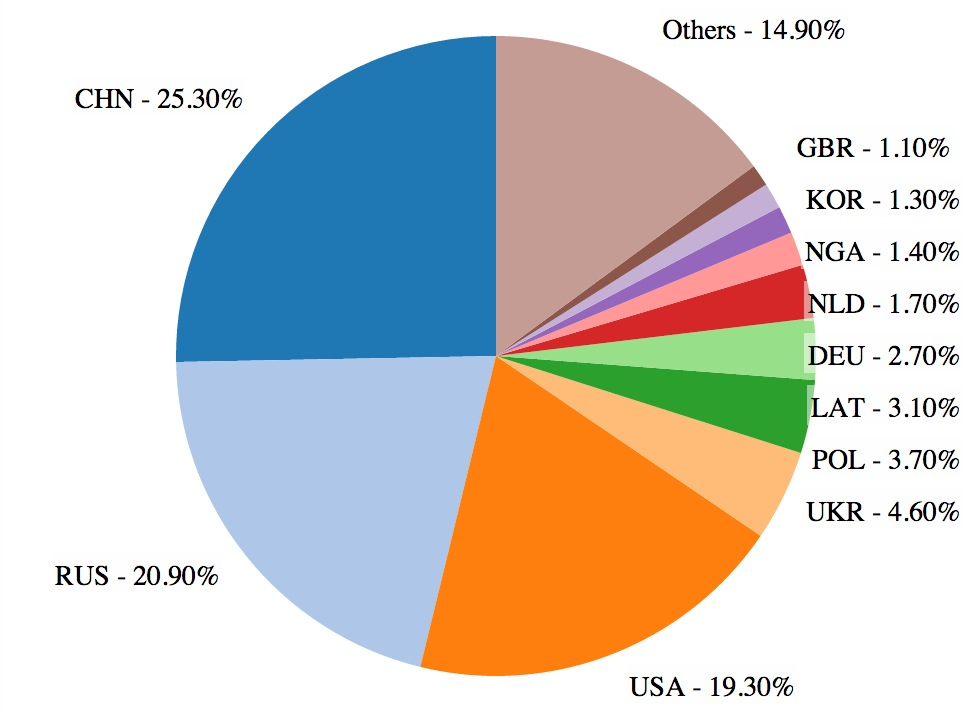
\includegraphics[scale=0.5]{Images/requests_countries.jpg}}
\caption{Number of requests divided by country\label{fig:requests_countries}}
\end{figure}

\subsubsection{Referer Analysis}

The analysis of the Referer HTTP header (whenever available) helped us identify how visitors were able to find our honeypots on the web. Based on the results, we can distinguish two main categories of users: criminals using search engines to find vulnerable ap- plications, and victims of phishing attacks following links posted in emails and public forums.
A total of 66,449 visitors reached our honeypot pages with the Referer header set. The domains that appear most frequently as referrers are search engines, followed by web mails and public forums. Google is leading with 17,156 entries. Other important search engines used by the attackers to locate our websites, were Yandex (1,016), a russian search engine, Bing (263), Microsoft search engine, and Yahoo (98). A total of 7,325 visitors arrived from web mail services (4,776 from SFR, 972 from Facebook, 944 were from Yahoo! Mail, 493 from Live.com, 407 from AOL Mail, and 108 from comcast.net). Finally, 15,746 requests originated from several public web forums, partially belonging to hacking communities, and partially just targeted by spam bots.

Finally, we extracted search queries (also known as ``dorks'', when used for malicious purposes) from Referer headers set by the most common web search engines. Our analysis shows that the search terms used by attackers highly depend on the application deployed on the honeypot. For example, the most common dork that was used to reach our Joomla web application contained the words \emph{``joomla allows you''}, while the Simple Machines Forum was often reached by searching \emph{``powered by smf''}. Our machine containing public web shells was often reached via dorks like \emph{``inurl:c99.php''}, \emph{``cyber anarchy shell''} or even \emph{``ftp AND brute-forcer AND security AND info AND processes AND mysql AND php-code AND en-coder AND backdoor AND back-connection AND home AND enumerate AND md5-lookup AND word-lists AND milw0rm AND itsearch AND self-kill AND about''}. The latter query, even though very long, was used more than 150 times to reach our machine with web shells. It was probably preferred to searching via \emph{``intitle:''} or \emph{``inurl:''} because attackers tend to customize names and titles of the scripts, therefore a search for direct text content may return more results. Some specialized search engines appear to be used as well, such as devilfinder.com \cite{devilfinder}, which was adopted in 141 cases to reach some of the shells on our machines. This search engine claims to show more low-ranking results than common search engines, not to store any search data, and to return up to 300 results on the same web page, making it very suitable for attackers willing to search for dorks and collect long lists of vulnerable websites.

\subsection{Reconnaissance}

